\begin{tikzpicture}[
	start chain=going right,
	diagram item/.style={
		minimum width=80pt,
%		minimum height=45pt,
		on chain,
		join
	}
]
\node [
	diagram item,
  label=center:Internet
] {
\includegraphics{Cisco_BW/cloud}};

%\node [
%	continue chain=going below,
%	diagram item,
%	label=right:Router
%] {
\includegraphics{Cisco_BW/router}};

\node [
	start branch=1 going below right,
	diagram item,
	label={[align=center]left:Load\\Balancer\\Backup}
] (LB2) {
\includegraphics{Cisco_BW/distributed_director}};

\node [
	continue chain=going below left,
	diagram item,
	label={[align=center]right:Load\\Balancer}
] {
\includegraphics{Cisco_BW/distributed_director}};

\node [
	continue chain = going below right,
	diagram item,
	label={[align=center]right:Services in distrinbuted\\across the wind farm}
] (farm) {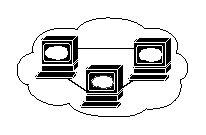
\includegraphics{Cisco_BW/web_cluster}};

\draw (LB2) -> (farm);

\node [
	start branch=1 going below right,
	diagram item,
	label=below:Http interface
] {\includegraphics{Cisco_BW/PC}};

\node [
	start branch=1 going below left,
	diagram item,
	label=below:OPC XML interface
] {\includegraphics{Cisco_BW/PC}};

\node [
	continue chain = going below,
	diagram item,
	label=below:Modbus interface
] {\includegraphics{Cisco_BW/PC}};

\end{tikzpicture}